\documentclass{beamer}

\mode<presentation>
{
  \usetheme{Singapore}
  \usecolortheme{rose}
  \setbeamercovered{transparent}
}

\usepackage[english]{babel}
\usepackage[latin1]{inputenc}
\usepackage{times}
\usepackage{listings}
\usepackage[T1]{fontenc} 
\usepackage{caption}
\usepackage{algorithm2e}

% Or whatever. Note that the encoding and the font should match. If T1
% does not look nice, try deleting the line with the fontenc.
\usepackage{amsmath}
\newcommand{\linespace}{\vskip 0.25cm}

\definecolor{MyForestGreen}{rgb}{0,0.7,0} 
\newcommand{\tableemph}[1]{{#1}}
\newcommand{\tablewin}[1]{\tableemph{#1}}
\newcommand{\tablemid}[1]{\tableemph{#1}}
\newcommand{\tablelose}[1]{\tableemph{#1}}

\definecolor{MyLightGray}{rgb}{0.6,0.6,0.6}
\newcommand{\tabletie}[1]{\color{MyLightGray} {#1}}

\beamertemplatenavigationsymbolsempty

\addtobeamertemplate{navigation symbols}{}{%
    \usebeamerfont{footline}%
    \usebeamercolor[fg]{footline}%
    \hspace{1em}%
    \insertframenumber/\inserttotalframenumber
}

\lstset{language=Java, frame=single, showspaces=false, }

\title[Developmental plasticity in N-gram GP]{Thread Scheduler Efficiency Improvements \\ for Multicore Systems}

% Sub-titles are optional - uncomment and edit the next line if you want one.
% \subtitle{Why does sub-tree crossover work?} 

% The text in square brackets is the short version of your name(s) and will be used in the
% header/footer depending on your theme.
\author[DFrz]{Daniel Collin Frazier}

% The text in square brackets is the short version of your institution and will be used in the
% header/footer depending on your theme.
\institute[U of Minn, Morris]
{
  Division of Science and Mathematics \\
  University of Minnesota, Morris \\
  Morris, Minnesota, USA
}

% The text in square brackets is the short version of the date if you need that.
\date[November '17, UMM, Minnesota] % (optional)
{18 November 2017 \\ UMM, Minnesota}

% Delete this, if you do not want the table of contents to pop up at
% the beginning of each subsection:
\AtBeginSection[]
{
	\begin{frame}<beamer>
		\frametitle{Outline}
		\tableofcontents[currentsection, hideothersubsections]
	\end{frame}
}

\begin{document}

\begin{frame}
\titlepage
\end{frame}

% For a 20-25 minute senior seminar talk you probably want something like:
% - Two or three major sections (other than the summary).
% - At *most* three subsections per section.
% - Talk about 30s to 2min per frame. So there should probably be between
%   15 and 30 frames, all told.

\section*{Introduction}

\subsection*{Introduction}

\begin{frame}
  \frametitle{Introduction}
  
\begin{itemize}
	\item \emph{Thread scheduler:} system component that manages the processing programs receive in a given time
  	\item Always running, so it must be efficient
  	
	\linespace
	
	\item Pre-2000 single-core era, scheduling was easy 
	\item Before multiple-core architecture, problem considered solved by Linux community
\end{itemize}
\end{frame}


\begin{frame}

\begin{figure}

\begin{quote}
``...not very many things ... have aged as well as the scheduler. Which is just another proof that scheduling is easy.''
\end{quote}
Linus, Torvals, 2001 \cite{Lozi:2016}
\end{figure}
\end{frame}

\begin{frame}
\frametitle{Introduction}

\begin{itemize}
\item Popular hardware changed rapidly throughout the 2000s

\linespace

\item Increasing affordability and adoption of multicore systems

\linespace

\item These developments complicated thread scheduler implementation

\linespace

\item Unfortunately, this complexity led to bugs that have been present for a decade
\end{itemize}
\end{frame}

\begin{frame}
\frametitle{A Decade of Wasted Cores}

\begin{columns}
\begin{column}{0.72\textwidth}
\begin{itemize}
\item Lozi et al. found four bugs in the Linux thread scheduler and fixed them~\cite{Lozi:2016}

\linespace

\item Previously undetected, required the development of new tools to notice them

\end{itemize}
\end{column}
\begin{column}{0.28\textwidth} %Why does to[p] make the figure on the bottom and [b]ottom make the figure on the top.....
\begin{figure}
\centering
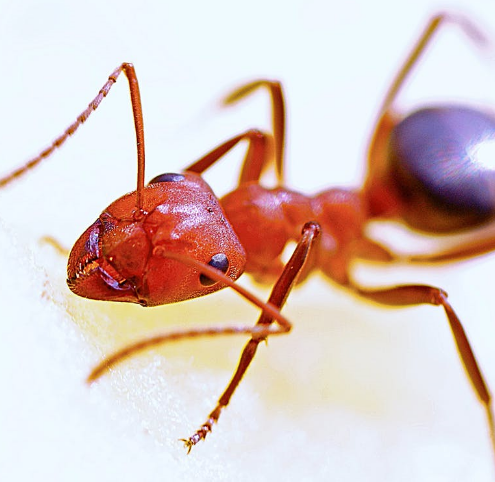
\includegraphics[width=0.95\textwidth]{Illustrations/ant_from_pexels.png}
\caption*{https://goo.gl/3wsfVU}
\end{figure}

\end{column}
\end{columns}

\end{frame}

\begin{frame}
\frametitle{A Decade of Wasted Cores}


\begin{itemize}

\item Lozi et al. compared performance benchmarks ran on \textbf{buggy} and \textbf{fixed} Linux scheduler implementations

\item Below are average performance improvements

\linespace
\end{itemize}

\begin{table}
	\centering
	\begin{tabular}{| l | r |}
	\hline
	\textbf{Bug title} & \textbf{Improvement} \\ \hline
	The Scheduling Group Construction bug & 5.96x \\ \hline
	The Group Imbalance bug & 1.05x \\ \hline
	The Overload-on-Wakeup bug & 1.13x\\ \hline
	The Missing Scheduling Domains bug & 29.68x \\ \hline
\end{tabular}
\end{table}

\end{frame}

\subsection*{Outline}

\begin{frame}
  \frametitle{Outline}
  \tableofcontents[hideallsubsections]
\end{frame}

\section[Concepts]{Concepts}

\subsection[Threads]{Threads}

\begin{frame}
\frametitle{Processors}
	\begin{itemize}
	\item Responsible for executing code
	\linespace
	\item Contain a number of cores:
	\begin{itemize}
		\item \emph{Single-core processor} (one processing unit) 
		\item \emph{Multicore processor} (two or more processing units)
		\item \emph{Manycore processor} (~20 or more processing units)
	\end{itemize}
	\linespace
	\item A processor with multiple cores allows it to perform tasks concurrently on each core
	\end{itemize}
\end{frame}

\begin{frame}
\frametitle{Using Threads}

\begin{columns}
	\begin{column}{0.5\textwidth}
		\linespace
		\begin{itemize}
		\item Imagine you're using photoshop, but assume one thread
		\item Say you load a large image and perform an expensive filter operation
		\end{itemize}
		\end{column}
	\begin{column}{0.5\textwidth}
		\begin{figure}
		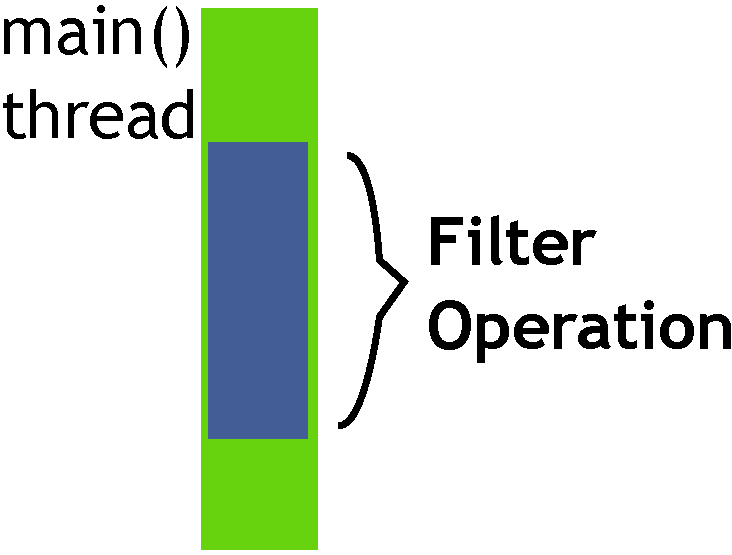
\includegraphics[width=0.95\textwidth]{Illustrations/ThreadExample_GUI_Part1}
		\label{fig:single_photoshop}
		\end{figure}
	\end{column}
\end{columns}

\end{frame}

\begin{frame}
\frametitle{Using Threads}


\begin{columns}
	\begin{column}{0.5\textwidth}
		\begin{itemize}
	
		\item \emph{Threads} allow programs to run multiple independent tasks concurrently	
		
		\linespace
		\linespace
		
		\item Useful for programs:
			\begin{itemize}
  			 \item with long, mostly-independent computations
			 \item with a graphical interface
	  		\end{itemize}
		\end{itemize}
	\end{column}
	
	\begin{column}{0.5\textwidth}
		\begin{figure}
		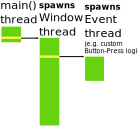
\includegraphics[width=0.95\textwidth]{Illustrations/ThreadExample_GUI_Part2}
		\label{fig:domains}
		\caption*{Example GUI Program. \\ \textbf{Three} threads are created within \textbf{one} process}
		\end{figure}
	\end{column}
\end{columns}

\end{frame}



\subsection[Locks]{Synchronicity and Locks}

\begin{frame}
\begin{center}
What if I ask you all a question right now?
\end{center}
\end{frame}

\begin{frame}
\frametitle{Synchronicity and Locks}

\begin{itemize}
	\item Control is achieved by employing locks
	
	\linespace
	
	\item \emph{Locks} secure objects or data shared between threads so that only one thread can read and write to it at one time

	\linespace

	\item When a thread \emph{locks} a lock it \textbf{acquires} the lock
	\item When a thread \emph{unlocks} a lock it \textbf{releases} the lock
\end{itemize}
\end{frame}

\subsection[Cache]{Thread State and Cache}

\begin{frame}
\frametitle{Process and Thread State}
\begin{itemize}
\item Process State

\begin{itemize}
	\item[] Resources shared amongst its multiple threads
\end{itemize}

\item Thread State
\begin{itemize}
	\item[] Scheduler uses this information to pause and resume a thread's execution
\end{itemize}

\linespace

\item Note: Process states are much heavier than thread states
\end{itemize}
\end{frame}

\begin{frame}
\frametitle{Context Switching}
\begin{itemize}
\item The scheduler \emph{switches} active threads on cores by saving and restoring thread and processor state information.
\item These switches are called \emph{context switches}
\end{itemize}
\end{frame}

\begin{frame}
\frametitle{Cache}

\begin{columns}
\begin{column}{0.5\textwidth}
\begin{itemize}
	\item Local copy of data designed for fast retrieval
	\item Hierarchical structure %POINT ON SLIDE L1, L2, Last-level cache
	\linespace
	\item Placement relative to core:
	\begin{itemize}
		\item on
		\item inside of
		\item outside

	\end{itemize}
\end{itemize}

\end{column}
\begin{column}{0.5\textwidth}
		\begin{figure}
		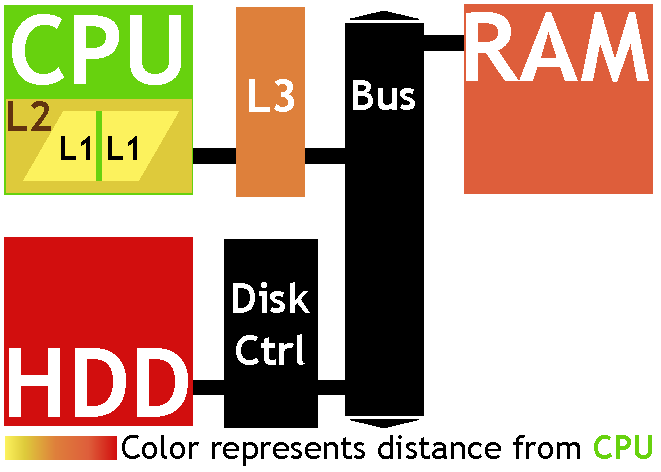
\includegraphics[width=0.95\textwidth]{Illustrations/CacheAbstract}
		\label{fig:domains}
		\caption{Distance of various forms of memory from CPU}
		\end{figure}
	\end{column}
\end{columns}
\end{frame}

\begin{frame}
\frametitle{Cache}

\begin{columns}
\begin{column}{0.5\textwidth}
\begin{itemize}
	\item \emph{Locality}: Speed of memory read and writes decrease as distance from CPU increases
	\item Cache is the fastest form of memory
	
	\linespace
	
	\item \emph{Cache coherence:} Any changes to memory shared by two caches must propogate to the other to maintain correctness
\end{itemize}

\end{column}
\begin{column}{0.5\textwidth}
		\begin{figure}
		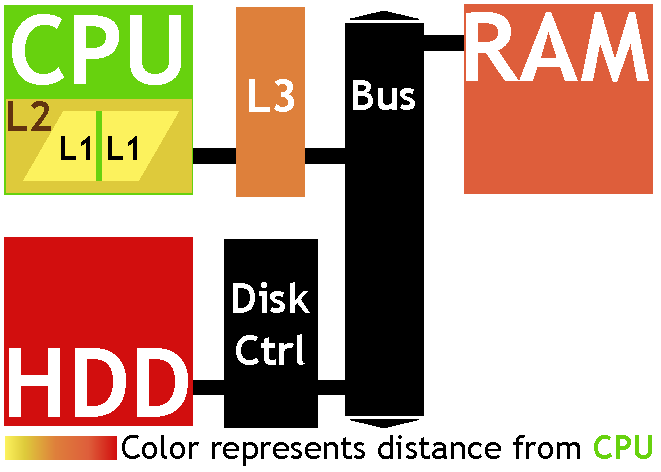
\includegraphics[width=0.95\textwidth]{Illustrations/CacheAbstract}
		\label{fig:domains}
		\caption{Distance of various forms of memory from CPU}
		\end{figure}
	\end{column}
\end{columns}
\end{frame}


\section[Thread Scheduling]{Thread Scheduling on Linux}
\subsection[CFS]{Completely Fair Scheduler}
\begin{frame}
\frametitle{Completely Fair Scheduler (CFS)}

\begin{itemize}
\item Default Linux thread scheduler (there are others)
\item Handles which threads are executed at what times on this core
\item Spend a \emph{fair} amount of runtime on all threads
\linespace

\item Designed with responsiveness and fairness in mind.


\end{itemize}
\end{frame}


\begin{frame}
\frametitle{Single-core Completely Fair Scheduler (CFS)}

\begin{itemize}
\item Runs on one core
\item Ensure all threads run \emph{at least once} within arbitrary interval of CPU~cycles
\item Distribute \emph{timeslices} (max CPU cycles) among threads
\item Threads with higher priority (weights) get larger timeslices

\end{itemize}

\begin{figure}
		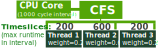
\includegraphics[width=0.8\textwidth]{Illustrations/CFS}
		\label{fig:cfs}
\end{figure}

\linespace

\end{frame}

\begin{frame}
\frametitle{CFS Runqueue}

\begin{itemize}
	\item Data structure containing threads
	\item Priority queue: sorts threads by number of cycles consumed in current interval
	\item When thread reaches its maximum cycles, preempted
\end{itemize}

\end{frame}

\begin{frame}
\frametitle{Runqueues on Multiple Cores}

\begin{itemize}

	\item Process states heavier than thread states, so context switches between threads of different processes are more expensive

	\linespace

	\item If cores shared a runqueue, access and changes need to be synchronous and cache-coherent
	\item Would slow the system to crawl
	\item So each core has its own runqueue and threads
\end{itemize}

\linespace

\begin{itemize}
\item Load on each of the core's runqueues must stay balanced
\item CFS periodically runs a load-balancing algorithm
\end{itemize}
\end{frame}

\section[New Schedulers]{Two New Schedulers}

\begin{frame}
\frametitle{Shuffler and FLSCHED}
\begin{itemize}
\linespace

\item Both schedulers aim to solve the same problem, but for different architectures

\linespace

\item \textbf{Problem:} Adding more threads to certain parallel computing applications on CFS makes the application operate slower rather than faster!

\linespace

\item Architectures:
\end{itemize}
\begin{table}
\begin{tabular}{l c l}
Shuffler & $\rightarrow$ & \textit{multiprocessor multicore} \\
FLSCHED & $\rightarrow$ & \textit{single-chip manycore processor}\\
\end{tabular}
\end{table}

\end{frame}

\subsection{Shuffler}
\begin{frame}
\frametitle{Shuffler}

\begin{itemize}


\item Researchers Kumar et al. measured lock times of massively parallel applications
\item \emph{Lock times}: amount of time process spends waiting for locks

\linespace

\item Found that massively parallel shared-memory programs experienced high lock times.


\end{itemize}

\end{frame}

\begin{frame}
\frametitle{Lock Contention}

\begin{itemize}



\item When two threads repeatedly contend for one lock, both threads are frequently waiting for each other to release
\linespace
\item If the two threads are located on separate processors, this problem is compounded by reduced locality
\linespace
\item Further, when both of the threads repeatedly modify the data corresponding to their lock, the cache of both processors must continue to update each other
\linespace
\item High \emph{lock contention}

\end{itemize}

\end{frame}


\begin{frame}
\frametitle{Shuffler}
\begin{itemize}
	\item CFS not mindful of lock contention or parent processes when choosing cores for threads
	
	\item Kumar et al. wanted to create a scheduler that did!
	\item Used Solaris scheudler as base
	\linespace
	\item \textbf{Strategy}: Migrate threads whose locks are contending near each other
	\linespace
	
	\item How do you determine which threads' locks are contending?
	\item Contending threads have similar lock acquisition times
	
\end{itemize}
\end{frame}

\begin{frame}
\begin{algorithm}[H]
	\SetKwInOut{Input}{input}\SetKwInOut{Output}{output}
	\Input{N: Number of threads;\\
	C: Number of Processors.}

	\Repeat{application terminates}{
		$\textbf{i. Monitor Threads}$ -- sample lock times of N threads.\\
		\If{lock times exceed threshold}{
			$\textbf{ii. Form Thread Groups}$ -- sort threads according to lock times and divide them into C groups. \\
			$\textbf{iii. Perform Shuffling}$ -- shuffle threads to establish newly computed thread groups.
		}
	}		
\end{algorithm}
\end{frame}

\begin{frame}
\frametitle{Shuffler Performance}

\begin{itemize}
\item Kumar et al. compared the efficiency of Shuffler vs Solaris scheduler
\item Used programs from four benchmarks to gather data.

\begin{columns}

\begin{column}{0.5\textwidth}
\begin{table}
	\centering
	\begin{tabular}{| c | r |}
	\hline
	\textbf{Program} & \textbf{\% Improvement} \\ \hline
	\emph{BT} & 54.1\% \\ \hline
		\emph{SC} & 29.0\% \\ \hline
		\emph{RX} & 19.0\% \\ \hline
		\emph{JB} & 14.0\% \\ \hline
		\emph{OC} & 13.4\% \\ \hline
		\emph{AL} & 13.2\% \\ \hline
		\emph{AS} & 13.0\% \\ \hline
		\emph{PB} & 13.0\% \\ \hline
		\emph{VL} & 12.8\% \\ \hline
		\emph{FS} & 12.0\% \\ \hline
		
\end{tabular}
\end{table}
\end{column}
\begin{column}{0.5\textwidth}
	\begin{table}
	\centering
	\begin{tabular}{| c | r |}
	\hline
	\textbf{Program} & \textbf{\% Improvement} \\ \hline
		\emph{FM} & 10.7\% \\ \hline
		\emph{AM} & 9.3\% \\ \hline
		\emph{GL} & 9.1\% \\ \hline
		\emph{EQ} & 9.0\% \\ \hline
		\emph{MG} & 8.8\% \\ \hline
		\emph{FA} & 6.0\% \\ \hline
		\emph{WW} & 5.2\% \\ \hline
		\emph{SM} & 4.7\% \\ \hline
		\emph{GA} & 4.0\% \\ \hline
		\emph{RT} & 4.0\% \\ \hline
\end{tabular}
\end{table}
\end{column}
\end{columns}
 
\end{itemize}

\end{frame}

\subsection{FLSCHED}
\begin{frame}
\frametitle{FLSCHED: The Lockless Monster}

\begin{itemize}
	\item Designed by Jo et al. with manycore processors in mind, particularly the Xeon Phi.


\linespace

\item The Xeon and Xeon Phi have 24 to 76 cores.
\linespace
\item One processor, so cache looks different than system that would use Shuffler
\linespace
\item With such parallelism, small pauses significantly reduce efficiency
\linespace

\item In the CFS, pauses come from locks necessitated by its features and requirements.

\end{itemize}
\end{frame}

\begin{frame}
\frametitle{One requirement to rule them all: EFFICIENCY!}

\begin{itemize}
\item FLSCHED Improves efficiency by removing all locks from the scheduler implementation

\item Gutted requirements and features of CFS and simplified
\linespace

\item Requirements they removed were \textbf{Fairness} and \textbf{Responsiveness}

\item Context switches requests delayed to reduce chance another thread steals the core in hope thread reactivates

\item Threads never forcefully preempt, instead join runqueue with high priority

\item Removed scheduler statistics reporting capabilities

\end{itemize}
\end{frame}


\begin{frame}
\frametitle{FLSCHED Performance}
\begin{itemize}

\item Like in Shuffler, used a benchmark of various problems.

\end{itemize}
\begin{figure}
\caption*{Operations per second (OPS) relative to CFS}
\centering
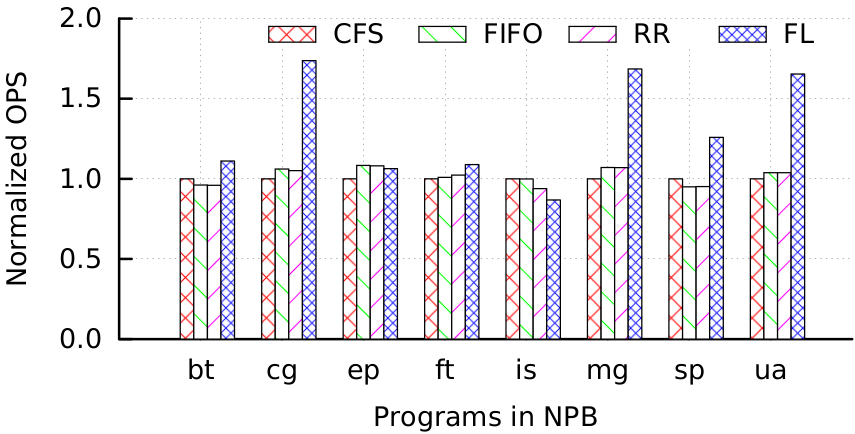
\includegraphics[width=0.95\textwidth]{Illustrations/FLSCHED_OPS.png}

\end{figure}
\end{frame}

\section[Conclusion]{Conclusion}

\begin{frame}
\frametitle{Conclusion}

\begin{itemize}
\item Thread scheduling is an important problem and becomes more relevant as number of cores increase

\linespace

\item System architecture can have surprising complexity in its effect on efficiency

\linespace

\item CFS tries to be the go-to scheduler for all problems, but can't

\item Does well, but when you need some extra push there are powerful alternatives available.

\end{itemize}
\end{frame}

\begin{frame}
\frametitle{Thanks!}

Thank you for your time and attention!

\begin{center}
{\huge Questions?}
\end{center}
\end{frame}

\section*{References}

\begin{frame} 
\frametitle{References} 

\begin{thebibliography}{lskdjf}

\bibitem{Jo:2017}
Jo, Heeseung and Kang, Woonhak and Min, Changwoo and Kim, Taesoo.
\newblock FLsched: A lockless and lightweight approach to OS scheduler for Xeon Phi.
\newblock In Proceedings of the 8th Asia-Pacific Workshop on Systems {\em3 APSys '17}, pages 8:1--8:8, Mumbai, India, 2017. ACM.

\bibitem{Kumar:2014}
K.~Kumar and P.~Rajiv and G.~Laxmi and N.~Bhuyan
\newblock Shuffling: A framework for lock contention aware thread scheduling for multicore multiprocessor systems
\newblock In 2014 23rd International Conference on Parallel Architecture and Compilation Techniques {\em3 PACT }, pages 289--300, 2014.

\bibitem{Lozi:2016}
Lozi, Jean-Pierre and Lepers, Baptiste and Funston, Justin and Gaud, Fabien and Qu{\'e}ma, Vivien and Fedorova, Alexandra
\newblock The {Linux} Scheduler: A Decade of Wasted Cores
\newblock In Proceedings of the Eleventh European Conference on Computer Systems {\em EuroSys '16}, pages 1:1--1:16, London, United Kingdom, 2016. ACM.

  
\end{thebibliography}

\linespace
\begin{center}
	See the GECCO '09 paper for additional references.
	\end{center}
\end{frame} 

\end{document}


